% \documentclass{beamer}
\documentclass[xcolor=dvipsnames]{beamer}
\usefonttheme{serif}
%% \usecolortheme[named=Blue]{structure}
\setbeamersize{text margin left=30mm, text margin right=30mm}
\useoutertheme{infolines}
%% \usetheme[height=7mm]{Rochester}
\usetheme{Pittsburgh}
\setbeamertemplate{items}[ball]
\setbeamertemplate{blocks}[rounded][shadow=true]
\setbeamertemplate{navigation symbols}{}

\usepackage[utf8x]{inputenc}
%% \usepackage{default}
\usepackage[english]{babel}
\usepackage{geometry}
%% \usepackage{fullpage}
\usepackage{amsmath, amsthm, amssymb}
\usepackage{listings}
\usepackage{pxfonts}
\usepackage{caption}


\captionsetup[figure]{labelformat=empty}

%% \usepackage{color}
%% \usepackage{graphicx}
%% \usepackage{natbib}
%% \usepackage{array}
%% \usepackage{booktabs}
%% \usepackage{tabu}
%% \usepackage[utf8]{inputenc}
%% \usepackage{fancyhdr}
%% \usepackage{float}
%% \usepackage{subfigure}
%% \usepackage{titlesec}

\setbeamertemplate{headline}{}
\setbeamertemplate{footline}[frame number]{}
\setbeamertemplate{navigation symbols}{}
\setbeamertemplate{footline}{}
\setbeamertemplate{footline}[frame number]

\setbeamertemplate{itemize items}{$-$}

\def\CCT{{C\nolinebreak[4]\hspace{-.05em}\raisebox{.4ex}{\tiny\bf ++}}}
\def\CC{{C\nolinebreak[4]\hspace{-.05em}\raisebox{.4ex}{\small\bf ++}}}


\definecolor{lstgray}{gray}{0.93}
\definecolor{strgray}{gray}{0.4}

\lstset{ %
  escapechar=@,
  language=C++,
  basicstyle=\footnotesize\ttfamily,
  %% basicstyle=\ttfamily,
  %% keywordstyle=\color{blue}\ttfamily,
  keywordstyle=\bfseries,
  stringstyle=\color{strgray}\ttfamily,
  commentstyle=\color{OliveGreen}\ttfamily,
  %% morecomment=[l][\color{red}]{\#},
  morecomment=[l][\color{blue}]{\#},
  backgroundcolor=\color{lstgray},
  %% keywordstyle=\color{red},
  frame=f,
  frameround=ffff,
  tabsize=2,
  breaklines=true,
  breakatwhitespace=false,
  showspaces=false,
  showstringspaces=false,
  xleftmargin=5pt,
  xrightmargin=5pt,
  morekeywords={in,out,ref,auto,inout,import,ushort,scope,exit,mixin,decltype,varid,sizeof,constexpr}
}

\def\redcolor{\color{red}}
\def\bluecolor{\color{blue}}
\def\blackcolor{\color{black}}
\def\graycolor{\color{gray}}
\def\greencolor{\color{OliveGreen}}


\def\sectionname{\translate{Section}}
\def\insertsectionnumber{\arabic{section}}
\setbeamertemplate{section page}
{
  \begin{centering}
    \begin{beamercolorbox}[sep=4pt,center]{part title}
      \usebeamerfont{section title}\insertsection\par
    \end{beamercolorbox}
  \end{centering}
}
\def\sectionpage{\usebeamertemplate*{section page}}


\AtBeginSection{\frame{\sectionpage}}


\title{Particulars}
\subtitle{(In the 21\textsuperscript{st} Century)}
\author{Dominic Jones}
\date{\small{August 2019}}
\institute{\small{University of Buckingham}}


\begin{document}


\begin{frame}[plain]
  \titlepage
\end{frame}


\begin{frame}[fragile]{General argument}
  \begin{itemize}
  \item I argue that unity, truth, and goodness are transcendental properties of being, whereas beauty is a \emph{derived} property from these three.\vspace{5mm}
  \item It is when \emph{we} see those three properties shining together in something, we call it \emph{beautiful}.\vspace{5mm}
  \item But to have some idea about transcendentals, first some ideas about \emph{particulars}, \emph{concepts} and \emph{universals} are would be helpful.
  \end{itemize}
\end{frame}


\begin{frame}[fragile]{This talk}
  \begin{itemize}
  \item There is a real distinction between primary and derived properties in substances.\vspace{5mm}
  \item \emph{(Somehow, by analogy, beauty is derived, whereas unity, truth and goodness are primary)}\vspace{5mm}
  \item Substances possess in a primary sense unity, truth and goodness, but artefacts only in a secondary sense.\vspace{5mm}
  \item \emph{(Somehow, by analogy, when we say an artefact is beautiful it is in a two-fold derived sense.)}\vspace{5mm}
  \end{itemize}
\end{frame}


\section{Aristotle's Categories}

\begin{frame}{Substance and nine accidents}
\begin{figure}
  \centering
  \begin{columns}
    \column{0.5\textwidth}
    \centering
    \caption {Substantial change}
    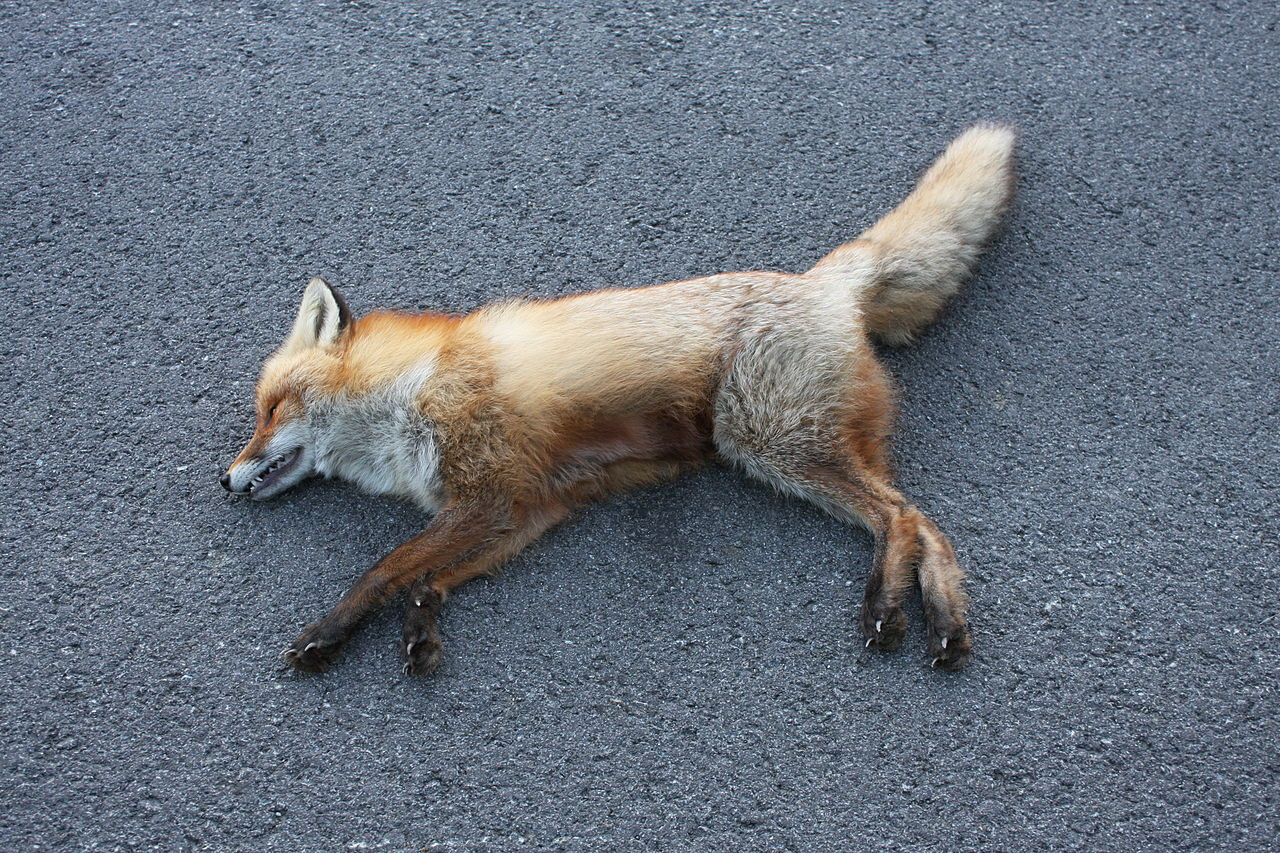
\includegraphics[width=0.99\textwidth]{fox}
    \column{0.5\textwidth}
    \centering
    \caption {Relational change}
    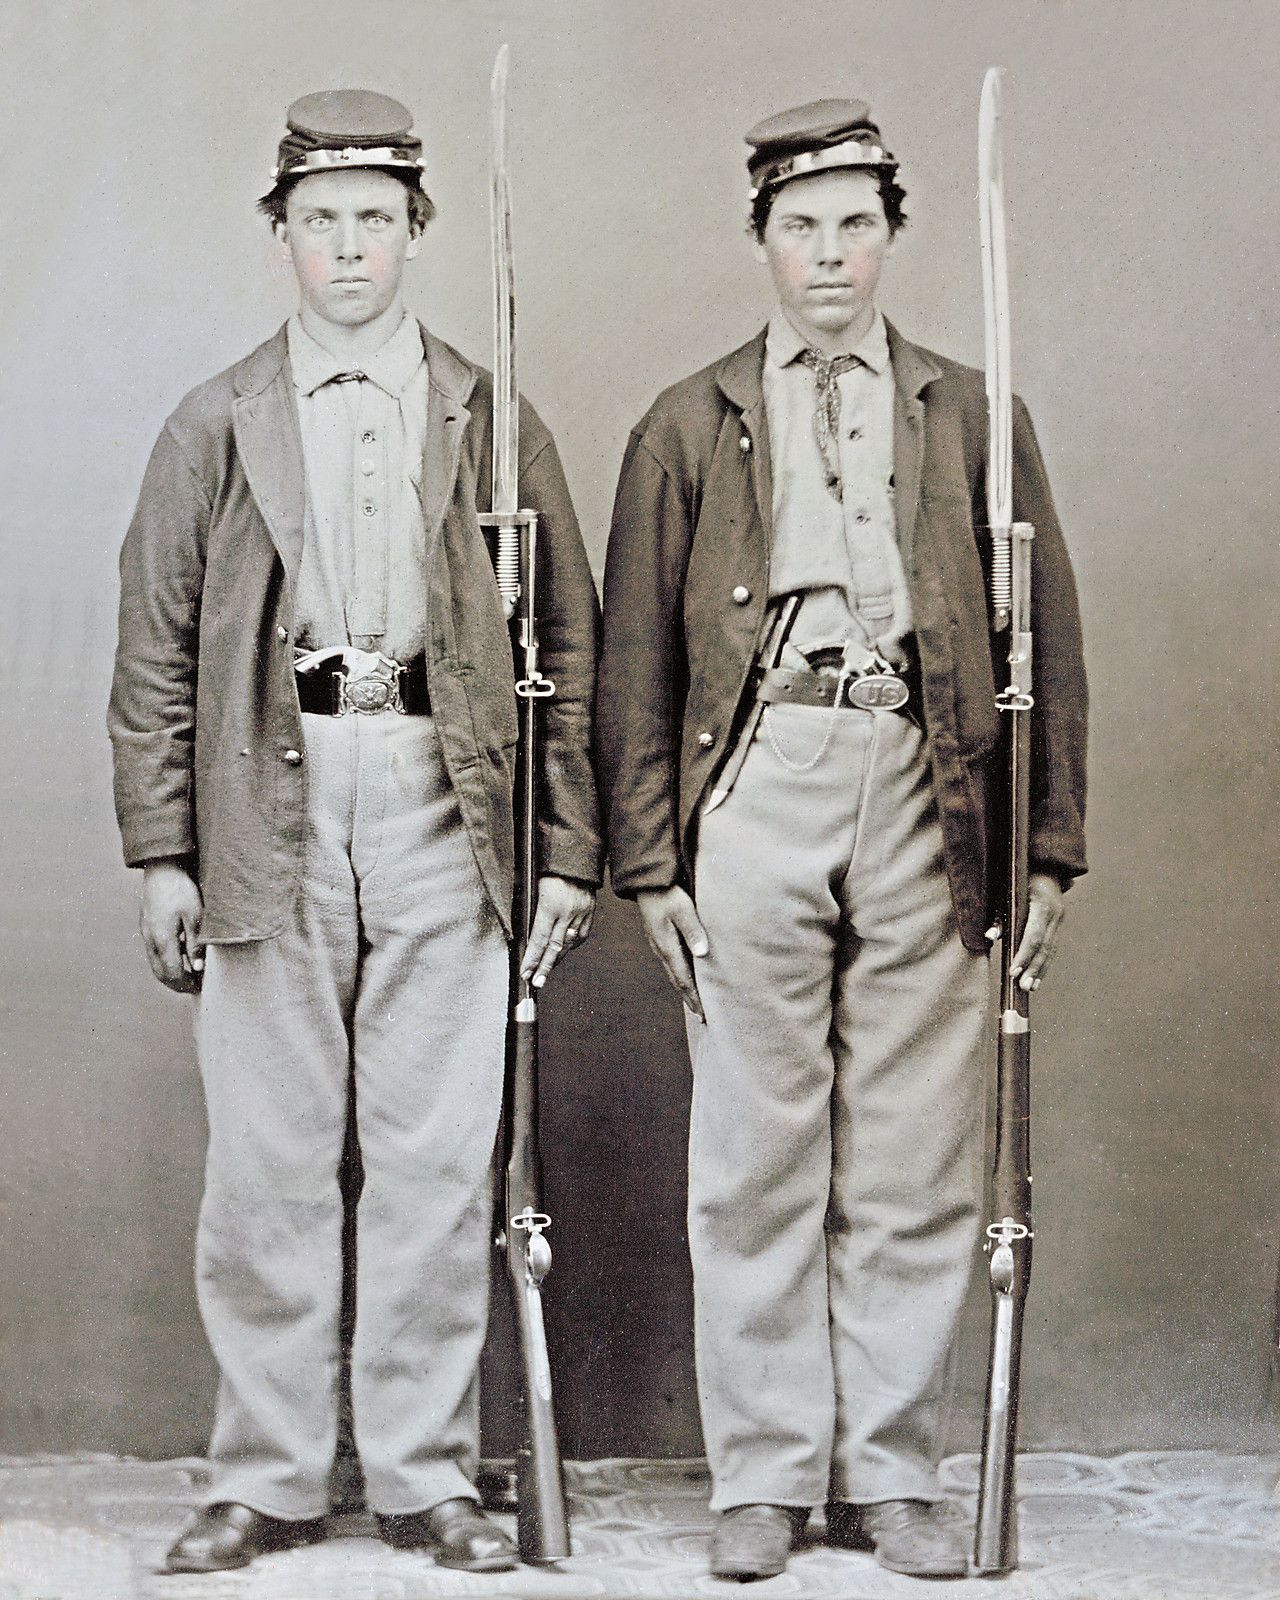
\includegraphics[width=0.9\textwidth]{relation}
  \end{columns}
\end{figure}
\end{frame}


\begin{frame}{Accidents are `present in' substances}
\begin{figure}
  \centering
  \begin{columns}
    \column{0.5\textwidth}
    \centering
    \caption {Quantitative change}
    
\includegraphics[width=0.99\textwidth]{cat}
    \column{0.5\textwidth}
    \centering
    \caption {Qualitative change}
    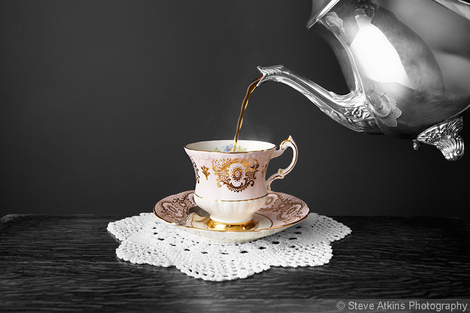
\includegraphics[width=0.99\textwidth]{tea}
  \end{columns}
\end{figure}
\end{frame}

\begin{frame}[fragile]{Primary and derived manners of being}
  \begin{itemize}
  \item The fox is dead. --- \emph{sub-stare} --- primary \vspace{5mm}
  \item The soldiers are brothers. --- \emph{esse ad} --- derived \vspace{5mm}
  \item The cat is fat. --- \emph{esse in} --- derived \vspace{5mm}
  \item The tea is cold. --- \emph{esse in} --- derived \vspace{5mm}
  \end{itemize}
\end{frame}



\section{Substances}


\begin{frame}[fragile]{Vegetative}
  \begin{columns}[T] % align columns
    %% \begin{column}{0.3\textwidth}
    %% \end{column}%
    %% \hfill%
    \begin{column}{0.99\textwidth}
      \begin{figure}[H]
        \centering
        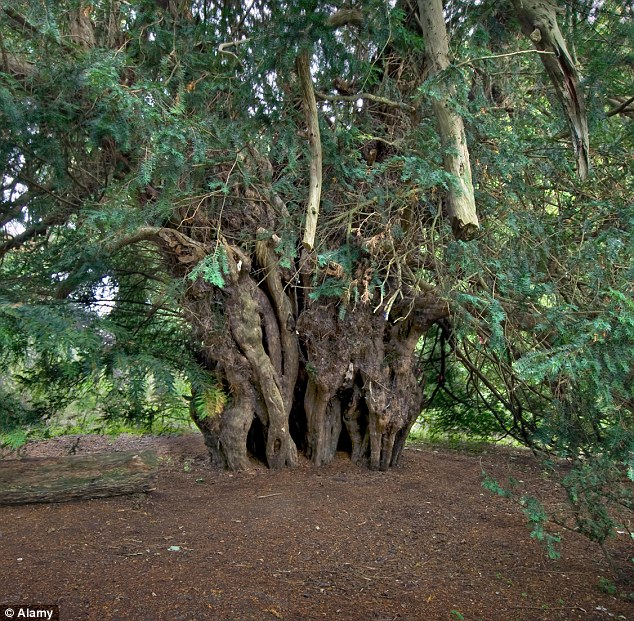
\includegraphics[width=0.7\textwidth]{ankerwyke-tree}
      \end{figure}
    \end{column}%
  \end{columns}
\end{frame}


\begin{frame}[fragile]{Sentient}
  \begin{columns}[T] % align columns
    %% \begin{column}{0.3\textwidth}
    %% \end{column}%
    %% \hfill%
    \begin{column}{0.99\textwidth}
      \begin{figure}[H]
        \centering
        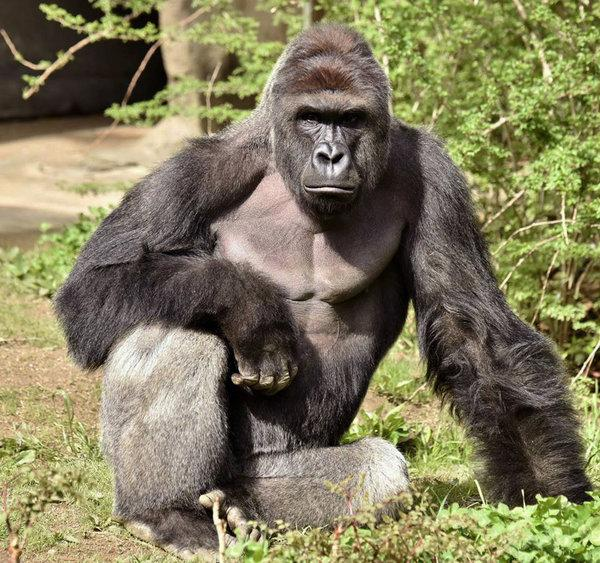
\includegraphics[width=0.7\textwidth]{gorilla}
      \end{figure}
    \end{column}%
  \end{columns}
\end{frame}


\begin{frame}[fragile]{Rational}
  \begin{columns}[T] % align columns
    %% \begin{column}{0.3\textwidth}
    %% \end{column}%
    %% \hfill%
    \begin{column}{0.99\textwidth}
      \begin{figure}[H]
        \centering
        
\includegraphics[width=0.9\textwidth]{wooster}
      \end{figure}
    \end{column}%
  \end{columns}
\end{frame}


\section{Artefacts}


\begin{frame}[fragile]{Organised parts}
  \begin{columns}[T] % align columns
    %% \begin{column}{0.3\textwidth}
    %% \end{column}%
    %% \hfill%
    \begin{column}{0.99\textwidth}
      \begin{figure}[H]
        \centering
        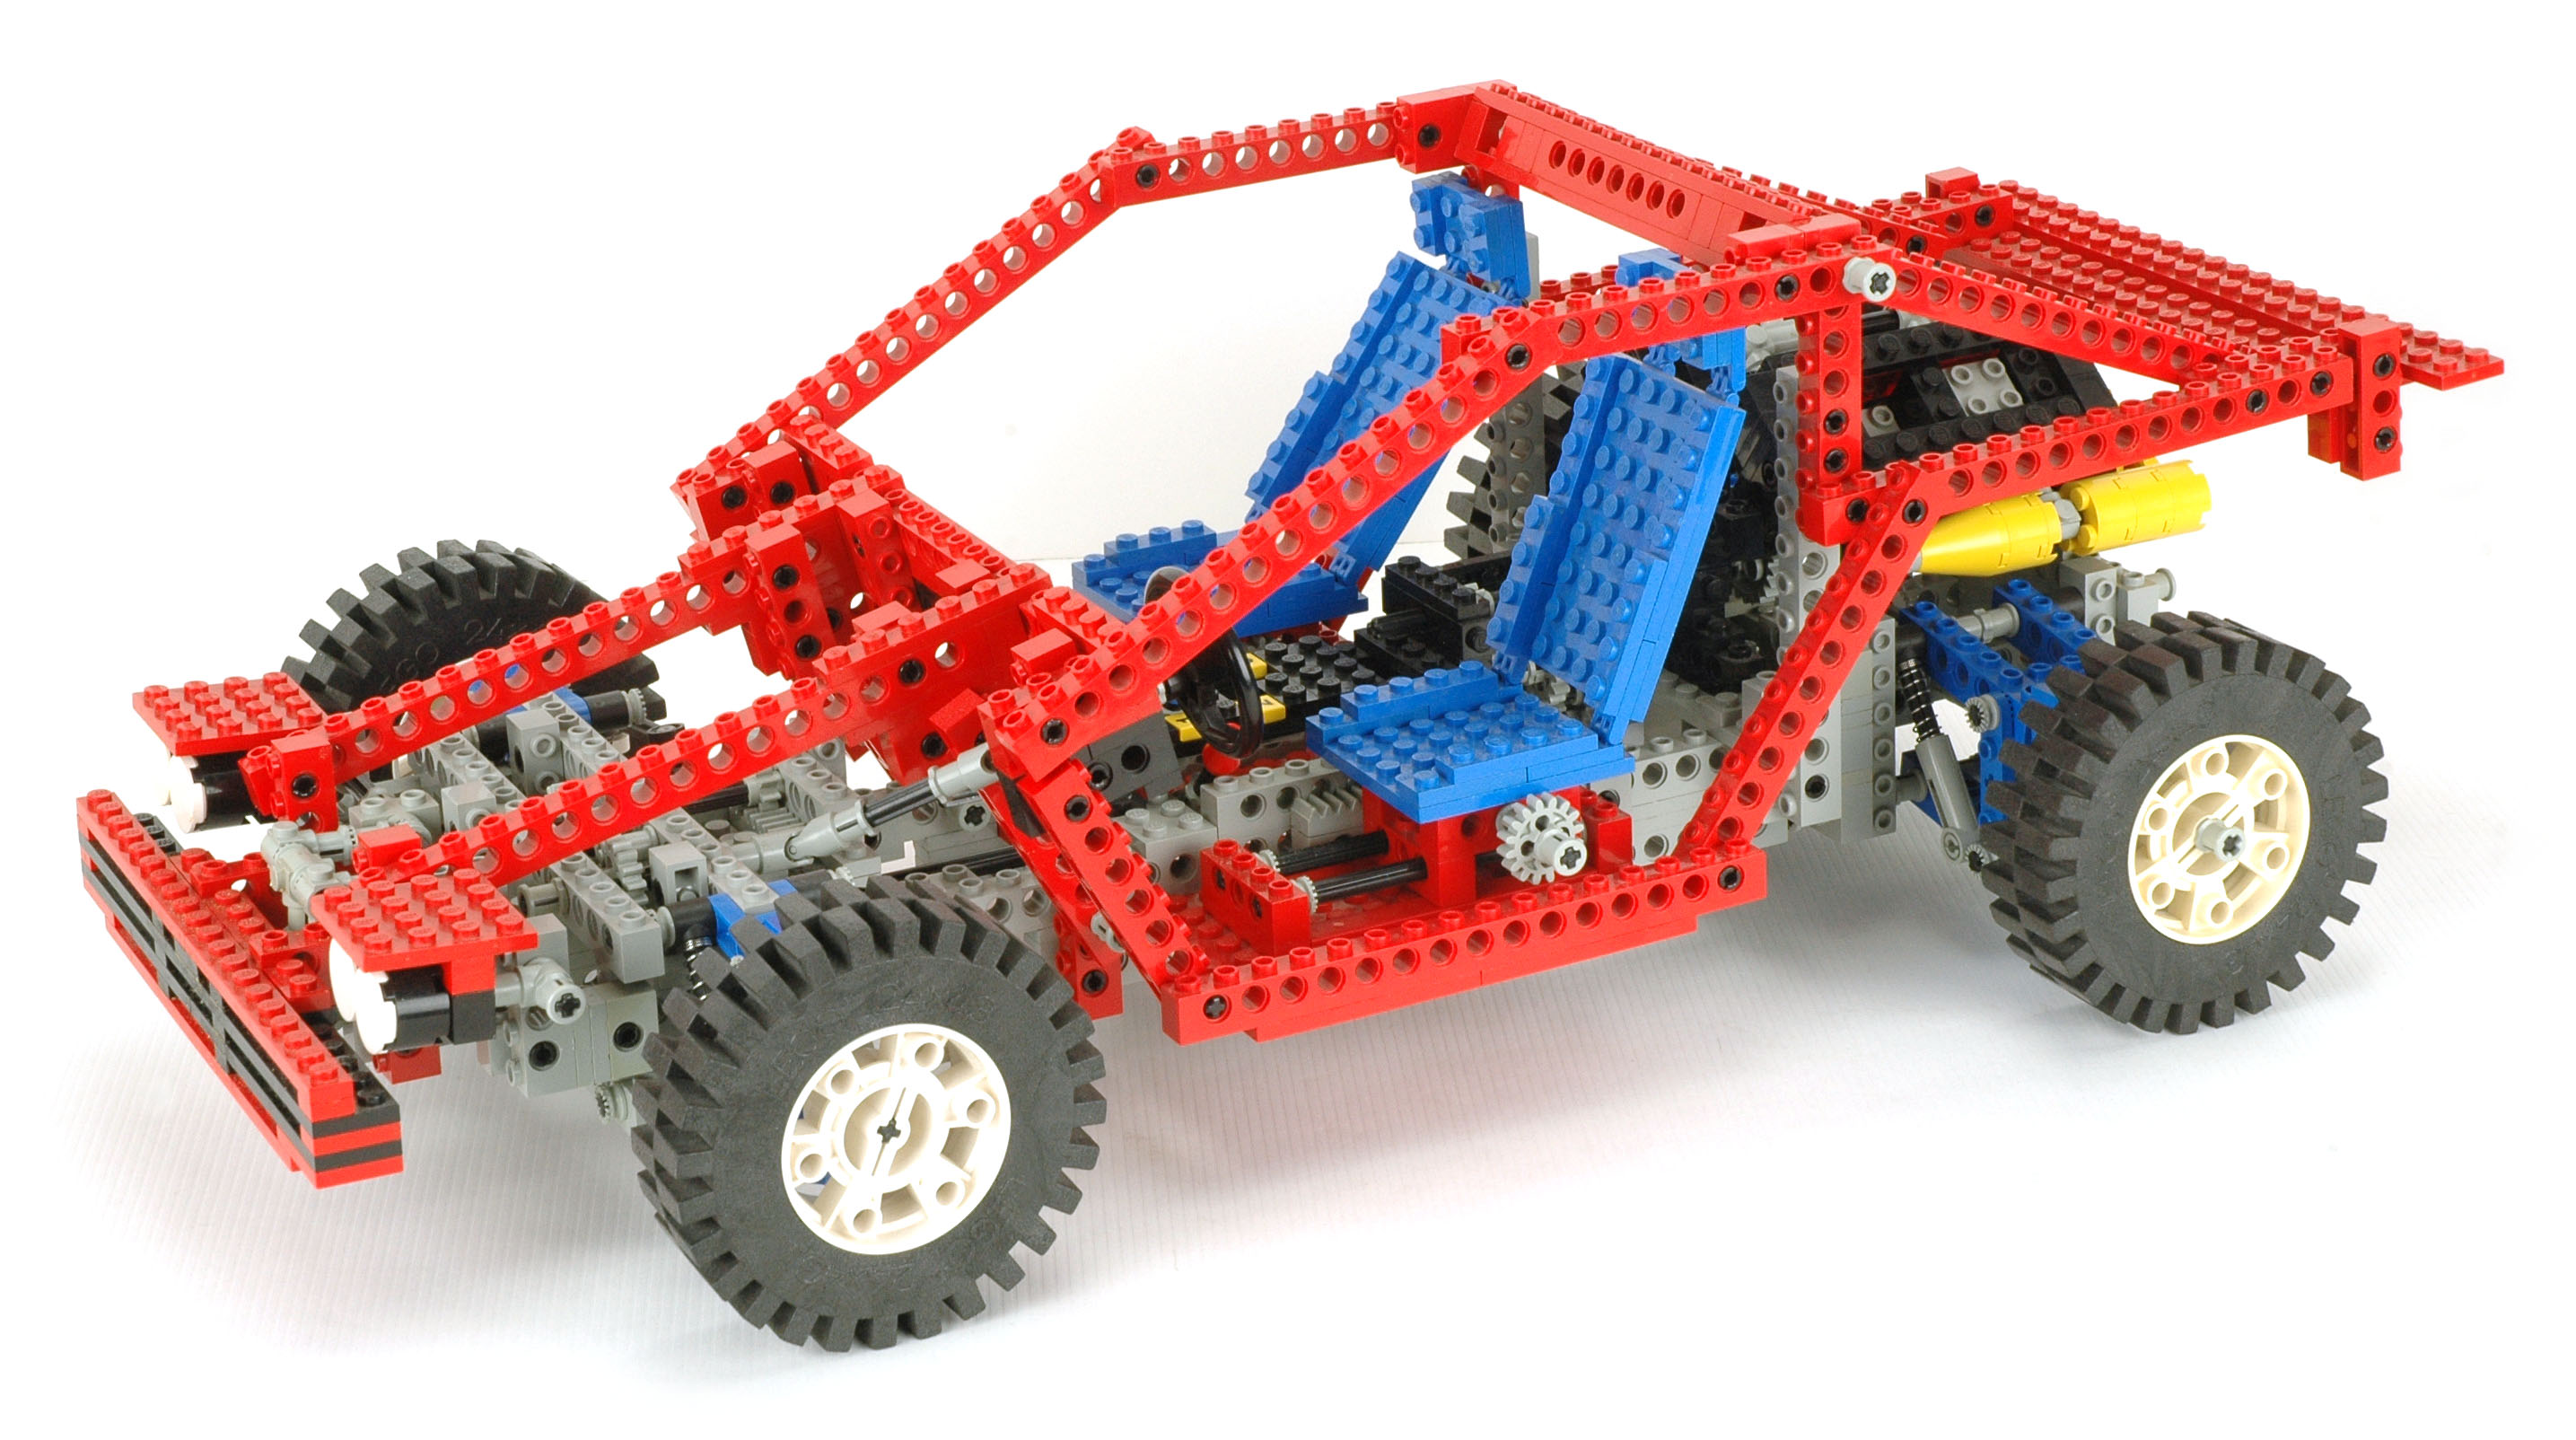
\includegraphics[width=0.9\textwidth]{1988_8865_car}
      \end{figure}
    \end{column}%
  \end{columns}
\end{frame}


\begin{frame}[fragile]{Formed substance}
  \begin{columns}[T] % align columns
    %% \begin{column}{0.3\textwidth}
    %% \end{column}%
    %% \hfill%
    \begin{column}{0.99\textwidth}
      \begin{figure}[H]
        \centering
        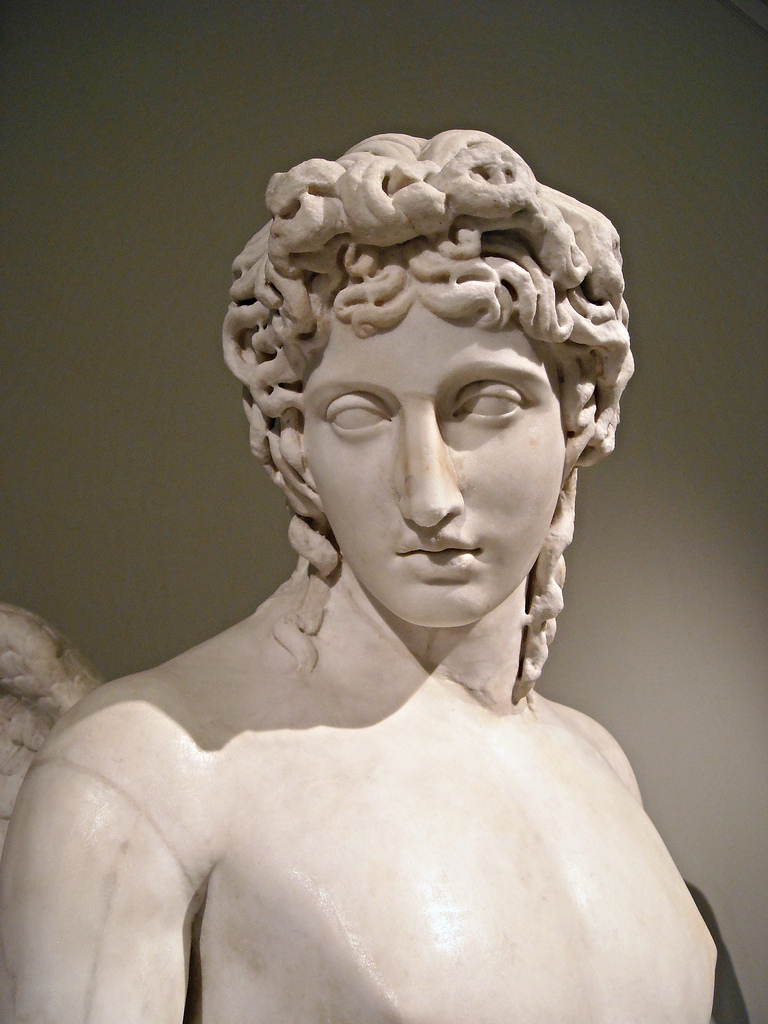
\includegraphics[width=0.6\textwidth]{eros}
      \end{figure}
    \end{column}%
  \end{columns}
\end{frame}


\section{Substance?}


\begin{frame}[fragile]{Artefact with inherent tendencies?}
  \begin{columns}[T] % align columns
    %% \begin{column}{0.3\textwidth}
    %% \end{column}%
    %% \hfill%
    \begin{column}{0.99\textwidth}
      \begin{figure}[H]
        \centering
        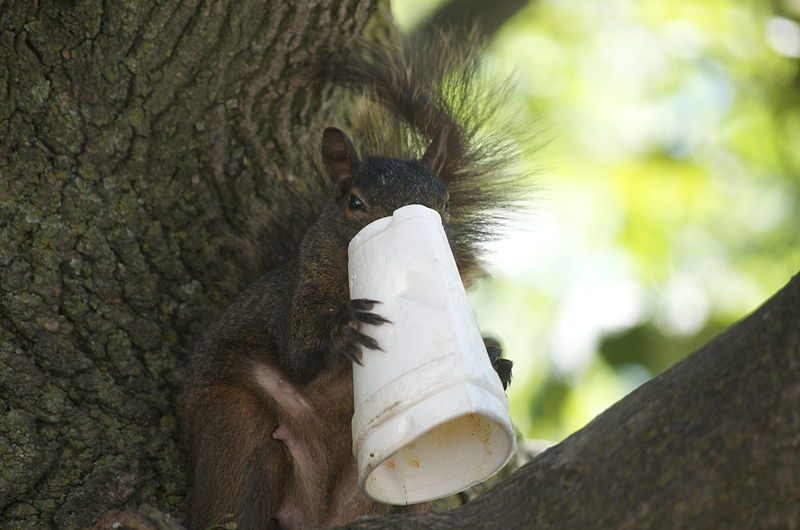
\includegraphics[width=0.9\textwidth]{styrofoam}
      \end{figure}
    \end{column}%
  \end{columns}
\end{frame}


\section{Artefact?}


\begin{frame}[fragile]{Substance with extrinsic tendencies?}
  \begin{columns}[T] % align columns
    %% \begin{column}{0.3\textwidth}
    %% \end{column}%
    %% \hfill%
    \begin{column}{0.99\textwidth}
      \begin{figure}[H]
        \centering
        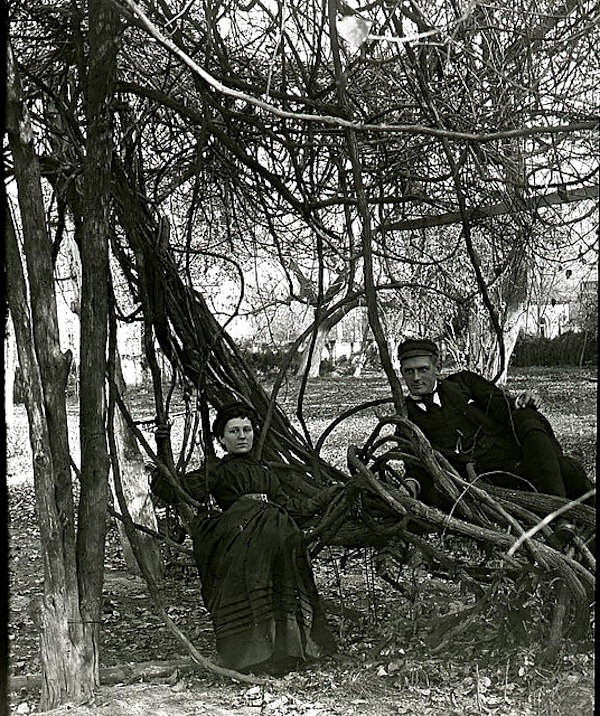
\includegraphics[width=0.6\textwidth]{vine-hammock}
      \end{figure}
    \end{column}%
  \end{columns}
\end{frame}


\begin{frame}[fragile]{Considerations}
  \begin{itemize}
  \item Substances have a `directedness' that comes from within --- it is intrinsic to it.\vspace{5mm}
  \item Artefacts have a directedness that comes from without --- it is extrinsic to it.\vspace{5mm}
  \item The unity of substances is unlike that of artefacts --- the latter can be reassembled.\vspace{5mm}
  \item The truth of substances is unlike that of artefacts --- the latter can be redefined.\vspace{5mm}
  \item The goodness of substances is unlike that of artefacts --- the latter can be repurposed.\vspace{5mm}
  \end{itemize}
\end{frame}


\begin{frame}[plain]
  \titlepage
\end{frame}

\end{document}
